\documentclass{article}% use option titlepage to get the title on a page of its own.
\usepackage{preamble}
\usepackage{hyperref}
\usepackage[toc,page]{appendix}
\usepackage[dvipsnames]{xcolor}
% \usepackage{titlesec}
\usepackage{float}
\usepackage{amsmath}
\usepackage{graphicx}

% \addbibresource{sample.bib}
\addbibresource{references.bib}
% \setcounter{secnumdepth}{4}
\graphicspath{{figures/}}

\usepackage{tikz}
\usetikzlibrary {decorations.pathmorphing, arrows.meta}
\usetikzlibrary {arrows.meta}

% drawing configuration

\newcommand{\tikzPicScale}{0.8}
\newcommand\streamW{1.25}
\newcommand\streamH{3.5}
\newcommand\padding{0.5}
\newcommand\filledColor{black!50}
\newcommand{\floatingStreamPath}[2]{
    (#1 + \streamW,#2)
    -- plot[domain=0:\streamH] ({#1 + 0.2 * sin((3 * \x + 3.15) r) + 0.2}, {#2 + \x})
    -- ({#1 + \streamW},{#2 + \streamH})
    -- cycle
}
\newcommand{\fixedStreamPath}[2]{
    (#1,#2) rectangle ({#1 + \streamW},{#2 + \streamH})
}
\newcommand{\streamSep}[2]{
    \draw[black, thick] ({#1 - 2}, #2) node[anchor=south west] {receive} node[anchor=north west] {pay} -- ({#1 + \streamW + \padding}, #2);
}

\title{Pendle Boros - an On-chain System \\ for Margin Interest Rate Swap Markets}
\author{Pendle Finance}

\date{\today}
\begin{document}
\maketitle

\section*{Abstract}
Interest rate swap markets play a crucial part in a financial system, as apparent from its relative size in Traditional Finance (TradFi).

In this paper, we present Pendle Boros - an on-chain system for capital-efficient interest rate swap markets for any kind of interest that has an on-chain oracle, including TradFi interest rates. This system complements Pendle V2 to allow for much higher capital efficiency in speculation and management of interests/yields.

\section{Overview}
There are several components of Pendle Boros, one building on top of another:
\begin{itemize}
    \item Interest rate swap accounting
    \item Interest rate trading zones and orderbook
\end{itemize}

The rest of the paper will discuss the components in details in chapter 2 and 3.

\section{Interest rate swap accounting}
\subsection{High level overview}
As with the traditional definition, an interest rate swap is an agreement between two parties to exchange one stream of interest payments for another over a set period of time.

This chapter describes a model for accounting the PnL of interest rate swaps among users, without regard for how the user can settle the profits and losses. These aspects will be discussed in Chapters 3.

There is always a \textbf{maturity} in the context of an interest rate swap.

In Pendle Boros, ``the system'' is always the direct counter-party to each user in the context of an interest rate swap. The system will make sure that the sum of all floating interest streams of all users is zero, such that the system takes zero exposure to interest rates fluctuations.

Central to Pendle Boros's interest rate swap mechanism is a \textbf{floating interest} on a \textbf{base asset} that fluctuates in real-time. For example, the short-term LIBOR rate on USD, the funding rates of ETHUSDT Perp market on Binance, or the stETH interest rate on stETH.

In Pendle Boros's interest rate swap, one interest stream is always the \textbf{floating rate}, which will be defined by an external oracle. The other interest stream is always a \textbf{fixed rate} that is specific to each interest rate swap position between a user and the system.

\subsection{Conceptualising interest rate swaps}
In this section, we discuss the two ways to conceptualize an interest rate swap position, which will become useful in thinking about the system.

We will use the example of a Binance ETH-USDT Perp Funding Rate market, expiring in 1 year, where the base asset is ETH.

\subsubsection{Floating interest streams and fixed interest streams}
A floating interest stream on x ETH represents the right to receive funding rate on x ETH over time, being paid in real-time as the funding rates are updated. An example of a tokenized version of a floating interest stream is the YT token in Pendle V2. 1 YT-stETH represents the right to receive the continuous yields on 1 stETH over time until a maturity.

A fixed interest stream of y\% on x ETH represents the right to receive y\% APR on x ETH, being paid in real-time together with the floating stream payments.

Figure \ref{fig:streams} shows a graphical representation of the two types of interest streams.

\begin{figure}
    \centering

    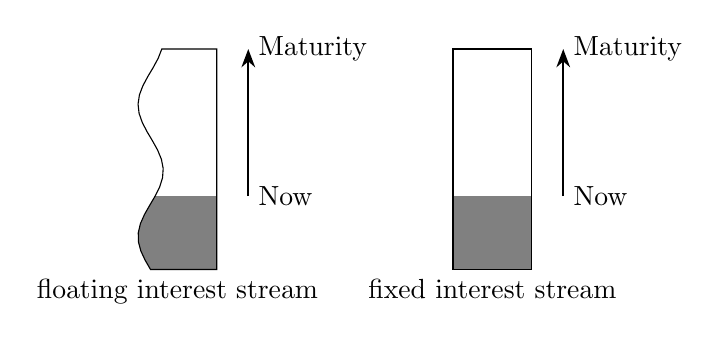
\begin{tikzpicture}[scale=\tikzPicScale]
        \newcommand{\filledLevel}{{\streamH / 3}}
        \begin{scope}
            \begin{scope}
                \path[clip] \floatingStreamPath{0}{0};
                \fill[\filledColor] (0,0) rectangle (\streamW, \filledLevel);
            \end{scope}
            \path[draw] \floatingStreamPath{0}{0};

            \draw[-Stealth, thick] (\streamW + \padding, \filledLevel) node[right] {Now} -- (\streamW + \padding, \streamH) node[right] {Maturity};
            \node[below] at ({\streamW / 2},0) {floating interest stream};
        \end{scope}

        \begin{scope}[shift={(5, 0)}]
            \begin{scope}
                \path[clip] \fixedStreamPath{0}{0};
                \fill[\filledColor] (0,0) rectangle (\streamW, \filledLevel);
            \end{scope}
            \path[draw] \fixedStreamPath{0}{0};

            \draw[-Stealth, thick] (\streamW + \padding, \filledLevel) node[right] {Now} -- (\streamW + \padding, \streamH) node[right] {Maturity};
            \node[below] at ({\streamW / 2},0) {fixed interest stream};
        \end{scope}
    \end{tikzpicture}

    \caption{Graphical representation of interest streams}
    \label{fig:streams}
\end{figure}

\subsubsection{Interest rate swap position - the traditional definition}
The traditional definition of an interest rate swap position is to exchange an interest stream for another interest stream.

There are only two types of interest rate swaps:
\begin{itemize}
    \item A fixed-to-float position, or a long rate position: receiving a floating interest stream and paying a fixed interest stream. Every time period, the user gets the floating interest payment and pays the fixed interest.
    \item A float-to-fixed position, or a short rate position: receiving a fixed interest stream and paying a floating interest stream. Every time period, the user pays the floating interest payment and receive the fixed interest.
\end{itemize}

Figure \ref{fig:swaps} shows a graphical representation of the two types of interest rate swaps. The black area represents the realised PnL over time.
\begin{figure}
    \centering
    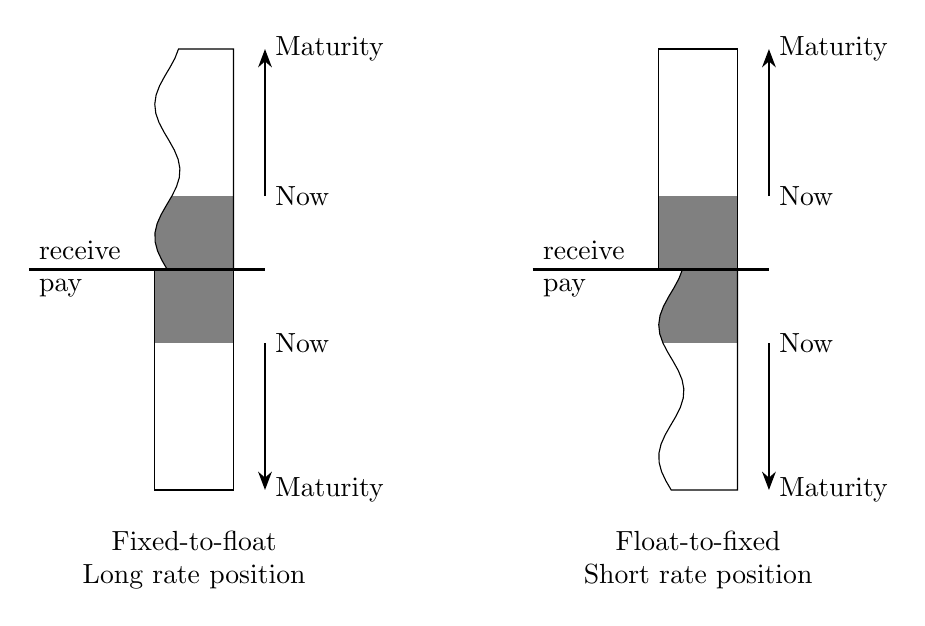
\begin{tikzpicture}[scale=\tikzPicScale]
        \newcommand{\filledLevel}{\streamH / 3}

        \begin{scope}
            \begin{scope}
                \path[clip] \floatingStreamPath{0}{0};
                \fill[\filledColor] (0,0) rectangle (\streamW, {\filledLevel});
            \end{scope}
            \path[draw] \floatingStreamPath{0}{0};
            \draw[-Stealth, thick] (\streamW + \padding, \filledLevel) node[right] {Now} -- (\streamW + \padding, \streamH) node[right] {Maturity};

            \begin{scope}
                \path[clip] \fixedStreamPath{0}{-\streamH};
                \fill[\filledColor] (0, 0) rectangle (\streamW, {-\filledLevel});
            \end{scope}
            \path[draw] \fixedStreamPath{0}{-\streamH};
            \draw[-Stealth, thick] (\streamW + \padding, {-\filledLevel}) node[right] {Now} -- (\streamW + \padding, -\streamH) node[right] {Maturity};

            \node[below, align=center] at ({\streamW / 2}, {-\streamH - \padding}) {Fixed-to-float\\Long rate position};

            \streamSep{0}{0};
        \end{scope}

        \begin{scope}[shift={(8, 0)}]
            \begin{scope}
                \path[clip] \fixedStreamPath{0}{0};
                \fill[\filledColor] (0,0) rectangle (\streamW, {\filledLevel});
            \end{scope}
            \path[draw] \fixedStreamPath{0}{0};
            \draw[-Stealth, thick] (\streamW + \padding, \filledLevel) node[right] {Now} -- (\streamW + \padding, \streamH) node[right] {Maturity};

            \begin{scope}
                \path[clip] \floatingStreamPath{0}{-\streamH};
                \fill[\filledColor] (0, 0) rectangle (\streamW, {-\filledLevel});
            \end{scope}
            \path[draw] \floatingStreamPath{0}{-\streamH};
            \draw[-Stealth, thick] (\streamW + \padding, {-\filledLevel}) node[right] {Now} -- (\streamW + \padding, -\streamH) node[right] {Maturity};

            \node[below, align=center] at ({\streamW / 2}, {-\streamH - \padding}) {Float-to-fixed\\Short rate position};

            \streamSep{0}{0};
        \end{scope}

    \end{tikzpicture}
    \caption{Graphical representation of interest rate swaps}
    \label{fig:swaps}
\end{figure}


\subsubsection{Interest rate swap position - buying/short selling a floating interest stream}
One observation is that when a swap is opened, we already know exactly how much the fixed stream will be worth: it is exactly
\begin{align*}fixedAPR \times notionalSize \times timeToMaturity\end{align*}

In Boros' contract system, to chose to realise the value of the fixed interest stream immediately when the swap is opened:
\begin{figure}[H]
    \centering
    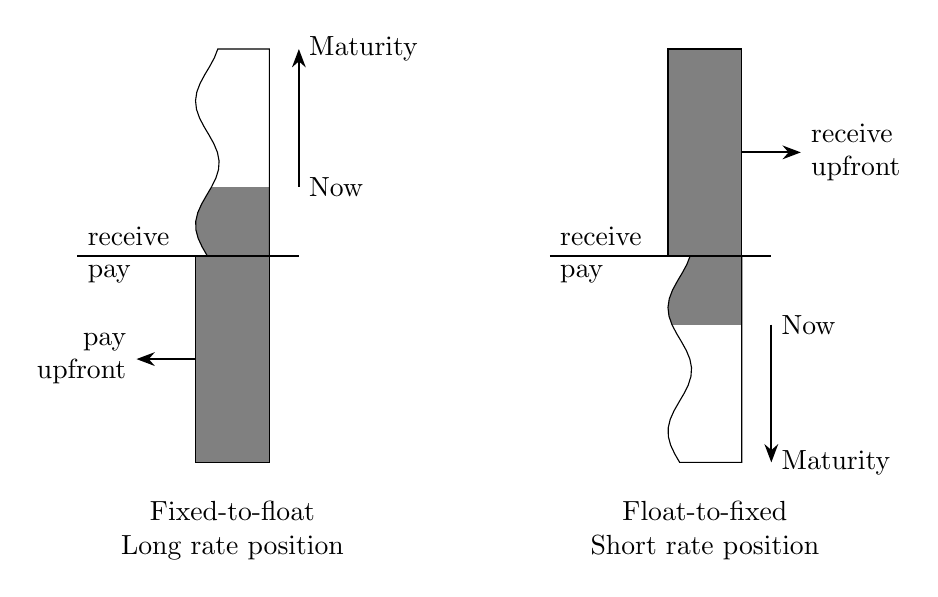
\begin{tikzpicture}[scale=0.75]
        \newcommand{\filledLevel}{\streamH / 3}

        \begin{scope}
            \begin{scope}
                \path[clip] \floatingStreamPath{0}{0};
                \fill[\filledColor] (0,0) rectangle (\streamW, {\filledLevel});
            \end{scope}
            \path[draw] \floatingStreamPath{0}{0};
            \draw[-Stealth, thick] (\streamW + \padding, \filledLevel) node[right] {Now} -- (\streamW + \padding, \streamH) node[right] {Maturity};

            \begin{scope}
                \path[clip] \fixedStreamPath{0}{-\streamH};
                \fill[\filledColor] (0, 0) rectangle (\streamW, {-\streamH});
            \end{scope}
            \path[draw] \fixedStreamPath{0}{-\streamH};
            \draw[-Stealth, thick] (0, {-\streamH / 2}) -- (-1, {-\streamH / 2}) node[anchor=east, align=right] {pay\\upfront};

            \node[below, align=center] at ({\streamW / 2}, {-\streamH - \padding}) {Fixed-to-float\\Long rate position};

            \streamSep{0}{0};
        \end{scope}

        \begin{scope}[shift={(8, 0)}]
            \begin{scope}
                \path[clip] \fixedStreamPath{0}{0};
                \fill[\filledColor] (0,0) rectangle (\streamW, \streamH);
            \end{scope}
            \path[draw] \fixedStreamPath{0}{0};
            \draw[-Stealth, thick] ({\streamW}, {\streamH / 2}) -- ({\streamW + 1}, {\streamH / 2}) node[anchor=west, align=left] {receive\\upfront};

            \begin{scope}
                \path[clip] \floatingStreamPath{0}{-\streamH};
                \fill[\filledColor] (0, 0) rectangle (\streamW, {-\filledLevel});
            \end{scope}
            \path[draw] \floatingStreamPath{0}{-\streamH};
            \draw[-Stealth, thick] (\streamW + \padding, {-\filledLevel}) node[right] {Now} -- (\streamW + \padding, -\streamH) node[right] {Maturity};

            \node[below, align=center] at ({\streamW / 2}, {-\streamH - \padding}) {Float-to-fixed\\Short rate position};

            \streamSep{0}{0};
        \end{scope}

    \end{tikzpicture}
    \caption{Upfront accounting of fixed rate streams}
    \label{fig:upfrontAccounting}
\end{figure}

\begin{itemize}
    \item When opening a fixed-to-float (long rate) position: the user pays the fixed interest debt immediately to obtain the floating interest stream. In a sense, the user ``buys'' the floating interest stream using a fixed amount of capital paid upfront. Over time, the user will receive the floating interest payments.
    \item When opening a float-to-fixed (short rate) position: the user receive upfront the fixed interest payments immediately, while incurring a debt of a floating interest stream. In a sense, the user borrows and sells the floating interest stream to get the capital upfront. Over time, the user needs to pay back the floating interest payments.
\end{itemize}

Figure \ref{fig:upfrontAccounting} shows a graphical representation of how the fixed stream's value is realised upfront in Boros' implementation.


\subsection{Notation} \label{notation}
\paragraph{time} $t$ represent time, in terms of years, from an arbitrary starting point (for example, Unix time 0 at 0 UTC 1 Jan 1970)
\paragraph{time delta} represent the duration between two legs distributions of the swap, in terms of fraction of a year. A duration of one day is corresponding to $\frac{1}{365}$
\paragraph{maturity} $t_{end}$ is the maturity of the interest rate swap
\paragraph{base asset} is the base asset whose interest is being exchanged in the interest rate swap
\paragraph{floating index} $floatingIndex(t)$ is how much 1 unit of \textbf{base asset} would have grown into from an arbitrary time $t_{start}$ until time $t$. This index defines the floating interest rates over time.
\paragraph{settlement fees} $F_{settlement}$ is a fees charged on all open interest rate swap positions, at every settlement every \textbf{time delta}. It is represented as a real number. A fees of 5\% will be represented by a value 0.05.

Note that in practice:
\begin{itemize}
    \item \textbf{floating index} is obtained from an oracle. For DeFi yield, this floating index could be exactly the ``exchangeRate'' like wstETH/stETH rate.
    \item \textbf{settlement fees} is stored in the system contract as a configuration. It could be changed by the governance. We denote $F_{settlement}(t)$ as the settlement fees at time $t$.
\end{itemize}

Let's define a system of interest rate swaps among a group of users $u$ from $u_1$ to $u_{N}$. Each interest rate swap market in this context is defined by a few parameters:
\begin{itemize}
    \item A specific \textbf{base asset}
    \item A specific \textbf{maturity} $t_{end}$ and \textbf{start time} $t_{start}$.
    \item The \textbf{floating interest} over time is specified via an increasing function $floatingIndex(t)$, with an arbitrary $t_{start}$.
\end{itemize}

Each \textbf{swap position} is defined by a few parameters:
\begin{itemize}
    \item \textbf{open time} $t_0$ is the timestamp where the swap is opened.
    \item \textbf{position size} $s(t)$ is the size of the user's floating stream at time $t$. A positive position where $s(t)>0$ means user $u$ is getting the \textbf{floating rate}, while $s(t)<0$ means the reverse. 
    \item \textbf{fixed rate debt} $debt(t)$ at time $t$ is the total obligation that the position needs to pay in its fixed rate leg. This obligation is conceptually ``realised'' every time a swap is open. It is as if the user has paid upfront all the fixed rate obligation.
    % \item \textbf{fixed rate} $f_{fixed}$ is how much fixed rate user $u$ will pay (if $s(t)>0$) or receive (if $s(t)<0$). This number could be negative, which means a user paying this rate (when $s(t)>0$) will in practice receive a positive payment. This rate is represented as an annualized number. For example, a 10\% fixed rate is represented by a value of 0.1.

\paragraph{sign} of a position size is either 1 for long, 0 for 0, or -1 for short.
\begin{align*}
    sign(s) &= \frac{s}{|s|}\\
    sign(0) &= 0
\end{align*}
\end{itemize}

\subsubsection{Realised profit and loss} \label{realisedPnL}

The \textbf{realised profit and loss} $p(t)$ of user $u$'s \textbf{position} at time $t$ is basically the \textbf{fixed rate debt}, the accumulated payments from the \textbf{floating rate} and the settlement fees, which we will define as:
    \begin{align}
        p_{realized}(t) &= -debt(t) +pFloat(t) + pFees(t) \\
        pFloat(t) &= \sum_{i=0}^{n-1}\left( floatingIndex(t_{i+1}) - floatingIndex(t_i) \right) \times s(t_{i+1}) \\
        pFees(t) &= -\sum_{i=0}^{n-1} | s(t_{i+1}) | \times F_{settlement}(t_{i+1}) \times (t_{i+1} - t_{i})
    \end{align}
    where $t_0 = t_{start}$ to $t_{n}=t$ are the discrete timestamps where the settlements happen. These discrete timestamps are mostly regular (for example, once every 8 hours, which means $t_{i+1} - t_{i}$ is always 8 hours), but \textbf{the frequency could change over time} based on the setting of the market (for example, a CEX perp funding rate frequency could change from every 8 hours to every 4 hours).

\textbf{What this means from the implementation perspective:}
\begin{itemize}
    \item Every ``settlement period'' of \textbf{time delta} (which is 8 hours for most funding rates for example), we update the current global floating index from an external oracle
    \item Along side the floating index, we also update a quantity called $feeIndex(t)$, which is the accumulated settlement fees from $t_{start}$ to $t$.
        \begin{align*}
            feeIndex(t) &= \sum_{i=0}^{n-1} F_{settlement}(t_{i+1}) \times (t_{i+1} - t_{i}) \\
                        &= feeIndex(t_{n - 1}) + F_{settlement}(t) \times (t_{n} - t_{n - 1})
        \end{align*}
    \item For each user, we keep track of the last floatingIndex since we ``touch their position'' (changing the position sizes)
    \item Since $s$ doesn't change for the user from $t_{last}$ to $t_{now}$, the changes in floating rate PnL ($pFloat$) and settlement fees PnL ($pFees$) are relatively simple to calculate:
    \begin{align}
        \Delta_{floatingPnL} &= s \times \left(floatingIndex(t_{now}) - floatingIndex(t_{last}) \right)\\
        \Delta_{settlementFeesPnL} &= - |s| \times (feeIndex(t_{now}) - feeIndex(t_{last}))
    \end{align}
    \item In implementation we \textbf{do not} need to store the total debt $debt(t)$, the total accumulated PnL from floating rate $pFloat(t)$ and the total accumulated PnL from settlement fees $pFees(t)$. Whenever we update the states for a user, we simply apply the changes to these numbers directly to the collateral of the user immediately.
    \begin{align}
        payment &= -anyNewDebt + \Delta_{floatingPnL} + \Delta_{settlementFeesPnL}\\
        collateral &= collateral + payment
    \end{align}
    \item Note how we don't need to keep track of the fixed rate of the position. Whenever a new position is opened, we realise these debt immediately into the collateral. In other words, the user pays (or receive) the total value of the fixed rate stream upfront.
\end{itemize}

The tuple $(t, floatingIndex(t), feeIndex(t))$ is known as the \texttt{FIndex} in our contract.

Every time user $u$ opens new position on this market, it's aggregated into his current position based on mechanism mentioned in \ref{merge}.

\subsection{State changes}
\subsubsection{The initial state}
At the start at time $t_0 \geq t_{start}$, for every user and market, their position has zero size and zero fixed rate debt:
    \begin{align*}
        s(t_0) = 0 \\
        debt(t_0) = 0 \\
    \end{align*}
The notation of user $u$ and market $M_i$ will be used when necessary (e.g. $s_u^{(i)}$ and $debt_u^{(i)}(t_0)$).
\subsubsection{Create a new pair of swaps}
The only state change possible in the accounting system for interest rate swaps is to create a new pair of interest rate swaps for two users $u_i$ and $u_j$ with the fixed rate $f_{new}$ and position size $s_{new}$ for $u_i$ and the same fixed rate $f_{new}$ and opposite position size $-s_{new}$ for $u_j$. 

When we talk about ``a swap with fixed rate $f_{new}$, position size $s_{new}$ opened at time $t$'', it is equivalent to ``a swap of position size $s_{new}$ and $debt_{new} = s_{new} \times t \times f_{new}$, opened at time $t$'', which is the standard way to represent swaps in our system. 

The existing position of each user will be merged with the newly created swap positions.
At any time $t > t_0$: (denote $t-$ as the moment right before $t$)
    \begin{align*}
        (s_{u_i}(t), debt_{u_i}(t)) &= mergeSwaps(s_{u_i}(t-), debt_{u_i}(t-), s_{new}, debt_{new})\\
        (s_{u_j}(t), debt_{u_j}(t)) &= mergeSwaps(s_{u_j}(t-), debt_{u_j}(t-), -s_{new}, -debt_{new})\\
    \end{align*}
As the \textbf{debt} is updated for both users, their realised PnL will be updated accordingly as well.

\textbf{Merging of two swaps} \label{merge}
When merging two swaps, we simply add the position sizes and debts:
    \begin{align*}
        mergeSwaps(s_1, debt_1, s_2, debt_2) &= (s_1+s_2, debt_1+debt_2)
    \end{align*}
\section{Interest rate swap trading zones and orderbooks}
\subsection{Overview}

In Pendle Boros, an \textbf{interest rate swap trading zone} is a collection of one or multiple ``interest rate swap markets'' with the same \textbf{base asset} (but the interest rates could be different or the \textbf{maturity} could be different or both could be different).

\textbf{Note:} In practice, for each base asset: there are multiple ``isolated zones'' consisting of only one market each (intended for more risky markets), and a cross-collateral zone comprised of the more bluechip markets.

To be able to open an interest rate swap, users will need to post some collateral in terms of \textbf{base assets} into the corresponding \textbf{interest rate swap trading zone} to guarantee that they can fulfill their obligations in the system (paying for potential negative PnL).

A user could open positions in multiple interest rate swap markets in the same interest rate swap trading zone, using the same amount of collateral.

To open a new interest rate swap, a user must have enough \textbf{initial margin} for the position they want to open.

To maintain all of their positions, their collateral must be enough to cover the unrealised profits and losses and the \textbf{maintenance margin} required for all of their positions. If the \textbf{current total position value} is below the required \textbf{maintenance margin},  the user can be liquidated by any other user.

As time passes, the realised profits and losses of a user's positions will be reflected in their collateral value.

There is also an orderbook integrated into each market of the trading zone.

The orderbook consists two sub-orderbooks: a positive orderbook consisting of orders with positive sizes, and a negative orderbook consisting of orders with negative sizes.

From the perspective of the interest rate swap accounting system (in chapter 2), the positive orderbook and the negative orderbook are just two users that might open swaps with other users and realise some profit and loss over time.

However, from the trading zone's perspective, the positive orderbook and the negative orderbook are not users. They don't have any collateral and don't get liquidated. Any open position, realised PnL and unrealised PnL by the orderbooks will implicitly count toward the open positions, realised PnL and unrealised PnL of users whose orders have been filled.

\subsection{Definitions}
\paragraph{Collateral value} $c_u(t)$ is the amount of \textbf{collateral} a user $u$ hold at time $t$ in the system, in terms of \textbf{base assets}. 

\paragraph{Interest rate swap (IRS) market} refers to a particular interest rate swap market. There are $n_M$ interest rate swap markets from $M_1$ to $M_{n_M}$. For each interest rate swap market $M_i$, \textcolor{red}{the unit to measure PnL/value is the \textbf{base asset}} and the positive value indicates gains.
\begin{itemize}
    \item The \textbf{maturity} is $t_{end}$.
    \item The \textbf{Oracle Mark rate} of the market at time $t$ is $r_m(t)$.
    \item The \textbf{initial margin (IM)} of a position of user $u$ in the market at time $t$ depends on their size and the margin of the open orders. The initial margin's formula is configured to control the risks in opening new positions in the system.
    \item The \textbf{maintenance margin (MM)} of a position of user $u$ in the market at time $t$ depends on their size. A position of \textbf{size} $s$ of user $u$ will have the maintenance margin of $MM(s, u, t)$ at time $t$. This function is configured to control the risks of open positions in the system.
\end{itemize}

\paragraph{Positive orderbook} Each IRS market has a \textbf{positive orderbook} that consists of $N^{+}$  orders in total, which are divided into a set $X_{open}^{+}$ of open orders, a set $X_{filled}^{+}$ of filled orders and a set $X_{settled}^{+}$ of settled orders. An order can move from the open set to the filled set and finally the settled set.
\begin{itemize}
    \item The total position size of the positive order book is $s^+$. This is the same as the total size of the orders in $X_{filled}^{+}$
    \item Each user $u$ have $N_u^{+}$ orders in total, each order $order_{u_i}$ have size $s_{u_i}^{+}$, fixed rate $f_{u_i}^{+}$ and filled timestamp $t_{u_i}^{+}$ (which is 0 if the order is not filled)
    \item The orders in the positive orderbooks are grouped into multiple ticks from  $k_{-Z}$ to $k_{Z}$, each tick consisting of orders with the same fixed interests.
    \item $Z$ is a constant for each market, which defines how many ticks there are in the orderbook ($2Z + 1$)
    \item The \textbf{tick interest} $I_{k_{i}}$ of tick $k_{i}$ follows an increasing function on integers
        \begin{align*}
            I_{k_{i}} = g(i)
        \end{align*}  
        \begin{center}
            where $g(0) = 0$ and $g(i) = -g(-i)$
        \end{center}
    An example of this function is:
        \begin{align*}
            g(i) &= (1+I_{smallest})^i-1\\
            g(-i) &= -g(i)\\
            i &\in N^*
        \end{align*}
        \begin{center}
            where $I_{smallest}$ is the interest rate of the first tick
        \end{center}
    \item As such, each order can only have certain fixed rates as defined by the ticks.
    \item The $N_u^{+}$ orders or user $u$ are divided into an open set $X_{open_{u}}^{+}$, a filled set $X_{filled_{u}}^{+}$ and a settled set $X_{settled_{u}}^{+}$. The Union of all users' open sets, filled sets and settled sets is basically the book's open set, filled set and settled set:
        \begin{align*}
            \sum_{u} N_u^+ &= N^+\\
            \bigcup_{u} X_{open_{u}}^{+} &= X_{open}^{+}\\
            \bigcup_{u} X_{filled_{u}}^{+} &= X_{filled}^{+}\\
            \bigcup_{u} X_{settled_{u}}^{+} &= X_{settled}^{+}\\
        \end{align*}
    \item Each order consumes a fixed ``pre-scaling initial margin'' amount that is set at the time when the order is placed, according to the pre-scaling initial margin function at the price of the order
        \begin{align*}
            pim_{u_i}^{+} = pim(s_{u_i}^{+}, f_{u_i}^{+}, t_{placed})
        \end{align*}
    \item Each user $u$ will have a \textbf{positive book pre-scaling initial margin} $pim^{+}_{u}(t)$ at time $t$, which is the sum of all pre-scaling initial margin of all \textbf{orders that have not been settled}.
        \begin{align*}
            pim^{+}_{u}(t) = \sum_{order_{u_i} \in X_{open_{u}}^{+}} pim_{u_i}^{+}   +   \sum_{order_{u_i} \in X_{filled_{u}}^{+}} pim_{u_i}^{+}
        \end{align*}
        \textbf{Note:} In practice, we always settle filled orders before calculating margin, so there will be no filled orders when calculating margin.
    \item The \textbf{total positive book size} of user $u$ is $b_{u}^{+}$, which is sum of the size of all unsettled orders in the positive orderbook:
        \begin{align*}
            b^{+}_{u}(t) = \sum_{order_{u_i} \in X_{open_{u}}^{+}} s_{u_i}^{+}   +   \sum_{order_{u_i} \in X_{filled_{u}}^{+}} s_{u_i}^{+}
        \end{align*}
        \textbf{Note:} In practice, we always settle filled orders before calculating margin, so there will be no filled orders when calculating margin.
    \item Each user $u$ will have an implicit position from each of their filled order $order_{u_i}\in X_{filled_{u}}^{+}(t)$ at time $t$, which gives $u$ a position of size $s_{u_i}^{+}$ and fixed rate debt $debt_{u_i}^{+}$. 
\end{itemize}

\paragraph{Negative orderbook} Each IRS market an a \textbf{negative orderbook} that works exactly like the positive orderbook. It consists of $N^{-}$  orders in total, which are divided into a set $X_{open}^{-}$ of open orders, a set $X_{filled}^{-}$ of filled orders and a set $X_{settled}^{-}$ of settled orders. The orders are also grouped into ticks from $k_{-Z}$ to $k_Z$. The concepts and formulas for each user $u$ are exactly the same, where the terms are: 
\begin{itemize}
    \item $u$ has $N_u^{-}$ orders in total, each order $order_{u_i}$ have size $s_{u_i}^{-}$, fixed rate debt $debt_{u_i}^{-}$ and filled timestamp $t_{u_i}^{-}$ (which is 0 if the order is not filled)
    \item The $N_u^{-}$ orders or user $u$ are divided into an open set $X_{open_{u}}^{-}$, a filled set $X_{filled_{u}}^{-}$ and a settled set $X_{settled_{u}}^{+}$
    \item The \textbf{negative book pre-scaling initial margin} is $pim^{-}_{u}(t)$ at time $t$
    \item The \textbf{total negative book size} of user $u$ is $b^{-}_{u}(t)$
    \item The total implicit combined position from all the filled orders in the negative orderbook has size $s_{u}^-(t)$ and fixed rate debt $debt_{u}^-(t)$
\end{itemize}

\paragraph{Combined implicit position from orderbooks} At any point in time, a user $u$ will have an implicit position of ($s_{u}^{book}(t), debt_u^{book}(t)) = mergeSwaps(s_{u_i}^{+}, debt_{u_i}^{+}, s_{u_i}^{-}, debt_{u_i}^{-}) $ at time $t$. This implicit position will have realised PnL $p_u^{book}$ and unrealised PnL $p_{unrealised}^{book}$ just like another user in the system.
\begin{itemize}
    \item The realised PnL as defined in Chapter \ref{realisedPnL}:
        \begin{align*}
            p^{book}(t) &= -debt^{book}(t) + pFloat(t) + pFees(t)
        \end{align*}
\textbf{Note:} In practice, the implicit position will always be merged into the user's standalone position first (by settling all filled orders) before we do any action that requires the calculation of realised or unrealised PnL.
\end{itemize}

\paragraph{For each user and a market}
\begin{itemize}
    \item For each user $u$ at time t:
        \begin{itemize}
            \item Their \textbf{standalone position size} is $s_{alone_u}(t)$
            \item Their standalone position's \textbf{fixed rate debt} is $debt_{alone_u}(t)$ at time $t$\\
            % \item Their \textbf{standalone realized PnL} at time $t$ is $p_{{alone_u}}$
            
            \textbf{Notes:} the total accumulated fixed rate debt defined here is for the sake of understanding the system and defining the model. In practice, we don't store this number because any new debt will just be realised into the collateral value of the user.
            \item Their \textbf{position size} $s_u(t)$ and \textbf{fixed rate debt} $debt_u(t)$ are the results from merging the standalone position $(s_{alone_u}(t), debt_{alone_u}(t))$ and the implicit position from the orderbooks $(s_{u}^{book}(t), debt_{u}^{book}(t))$ according to the mechanics in chapter 2.\\
            \textbf{Notes:} In our implementation, we always settle all user's filled orders before any on-chain action that needs the calculation of maintenance margin, so $s_u(t)$ and $debt_u(t)$ will be exactly the same as $s_{alone_u}(t)$ and $debt_{alone_u}(t)$ by then.
            \item Their \textbf{realized PnL} at time $t$ is $p_u$ which is the result from holding $(s_u(t), debt_u(t))$ over time. Any changes in realised PnL will be realised into the collateral value immediately.
                \begin{align*}
                    c_u(t) = c_u(t-) + p_u(t) - p_u(t-)
                \end{align*}
            \item Their \textbf{positive pre-scaling initial margin} at time $t$ $pim_{total_u}^+(t)$ is the pre-scaling initial margin consumed by positive orders and positions. This is 0 if the user is currently shorting rate and the total positive book size is not more than current position size.
            
            if $s_{alone_u} < 0$ and $b_{u}^{+} \leq |s_{alone_u}|$
                \begin{align*}
                    pim_{total_u}^+(t) = 0
                \end{align*}
            Else:
                \begin{align*}
                    pim_{total_u}^+(t) = pim^{+}_{u}(t) \pm pim(s_{alone_u}(t), r_m(t), t)
                \end{align*}
                \textbf{Note} It is + if $s_{alone_u} \geq 0$
            \item Their \textbf{negative pre-scaling initial margin} at time $t$ $pim_{total_u}^-(t)$ is the pre-scaling initial margin by negative orders and positions. This is 0 if the user is currently longing rate and the total negative book size is not more than current position size.
            
            if $s_{alone_u} > 0$ and $b_{u}^{-} \leq |s_{alone_u}|$
                \begin{align*}
                    pim_{total_u}^-(t) = 0
                \end{align*}
            Else:
                \begin{align*}
                    pim_{total_u}^-(t) = pim^{-}_{u}(t) \mp pim(s_{alone_u}(t), r_m(t), t)
                \end{align*}
                \textbf{Note} It is - if $s_{alone_u} \geq 0$
            \item Their \textbf{pre-scaling initial margin} is the bigger number between the two above
                \begin{align*}
                    pim_{u}(t) = \max( pim_{total_u}^+(t), pim_{total_u}^-(t)) 
                \end{align*}
            
            \item The \textbf{initial margin} consumed by the user at time $t$ is $im_u(t)$
                \begin{align*}
                    im_u(t) = IM\left(pim_{u}(t), u, t \right)
                \end{align*}\
            \item Their \textbf{normalised position size} is $s_{{norm}}(t)$ at time t
                \begin{align*}
                    s_{{norm_u}}(t) = s_u(t) \times (t_{end} - t)
                \end{align*}
            
  
            \item Their \textbf{unrealised PnL} at time $t$ is $p_{unrealized_u}(t)$ \\
                \begin{align*}
                    p_{unrealized_u}(t) = s_{{norm_u}}(t) \times r_m(t)
                \end{align*}\
             
            \item The \textbf{maintenance margin} for the position at time $t$ is $mm_u(t)$
                \begin{align*}
                    mm_u(t) = MM \left( s_u(t), u, t \right)
                \end{align*}  
            
        \end{itemize}
\end{itemize}

\paragraph{Total initial margin} consumed by all of a user $u$'s positions at time $t$ is $m^{total}_u(t)$. It is the sum of all the \textbf{initial margin} consumed across all the markets, in terms of the base asset.
    \begin{align*}
        im^{total}_u(t) = \sum_{i=1}^{n_M} im_u^{(i)}(t)
    \end{align*}

\paragraph{Total maintenance margin} required by all of a user $u$'s positions at time $t$ is $m^{total}_{{main}_u}(t)$. It is the sum of all the \textbf{maintenance margin} required across all the markets, in terms of the base asset.
    \begin{align*}
        mm^{total}_{u}(t) = \sum_{i=1}^{n_M} mm_u^{(i)}(t)
    \end{align*}

\paragraph{Current total value} of a user $u$ at time $t$ is the sum of their collateral value and all the unrealized profits and losses across all the markets
    \begin{align*}
        v_u(t) = c_u(t) + \sum_{i=1}^{n_M} p_{unrealized_u}^{(i)}(t)
    \end{align*}


\paragraph{Health ratio} of a user $u$ at time $t$ $healthRatio_u$ is the ratio between their \textbf{current total value} and their \textbf{total maintenance margin}
    \begin{align*}
        healthRatio_u(t) = \frac{ v_u(t) }{mm^{total}_{u}(t)}
    \end{align*}
A user is deemed \textbf{healthy} if their \textbf{health ratio} is larger than 1.

\paragraph{Fees} There are four fee factors related to 4 different types of fees in Boros:
\begin{itemize}
    \item \textbf{Settlement fees} $F_{settlement}$ as defined in chapter \ref{notation}
    \item \textbf{Taker fees} $F_{taker}$ is charged on market orders on the orderbook. It is represented as a real number. A fees of 5\% will be represented by a value of 0.05. Each user $u$ can have a taker fee factor $fee_{u_{taker}}$.
    \item \textbf{OTC swap fees} $F_{otc}$ is charged on public opening of swaps between any two users. It is represented as a real number. A fees of 5\% will be represented by a value of 0.05. Each user $u$ can have an otc fee factor $fee_{u_{otc}}$.\item \textbf{OTC swap fees} $F_{otc}$ is charged on OTC swaps between any two users. It is represented as a real number. A fees of 5\% will be represented by a value of 0.05. Each user $u$ can have an otc fee factor $fee_{u_{otc}}$.
    \item \textbf{liquidation fees} $F_{liq}$ is charged from the liquidator after a liquidation. It is represented as a real number. A fees of 5\% will be represented by a value of 0.05.
\end{itemize}

\textcolor{red}{The notation for market $M_i$ and user $u$ is omitted when the context does not require the market or user to be specified.}

\subsection{State changes}
$t-$ denotes the moment right before a state change at time $t$
\subsubsection{The initial state}
At the start at time $t_0$, for every user $u$ and every market $M_i$:
    \begin{align*}
        s_{alone_u}^{(i)}(t_0) &= 0\\
        debt_{alone_u}^{(i)}(t_0) &= 0\\
        p_{u}^{(i)}(t_0) &= 0\\
        p_{unrealized_u}^{(i)}(t_0) &= 0\\
    \end{align*}
For every user:
    \begin{align*}
        c_u(t_0) &= 0\\
        v_u(t_0) &= 0\\
    \end{align*}
\subsubsection{Add/remove collateral}
This is the only state change that an ``ineligible user'' can do. In the contract, ``becoming eligible'' is equivalent to entering the very first market. 

At any time $t$, a user $u$ can adjust their \textbf{collateral value} by $d_c$, as long as the \textbf{strict initial margin requirement} satisfies after the change.
    \begin{align*}
        c_u(t) &= c_u(t-) + d_c\\
    \end{align*}
After the change, the user must satisfy IM requirement of:
    \begin{align*}
        im_u^{total}(t) &\leq v_u(t)
    \end{align*}

\paragraph{Min deposit amount to become eligible} To become eligible (in the contract, its equivalent to entering the first market), the user must have deposited a minimum amount $MinDepositAmount$, which is a global setting per asset zone.

\subsubsection{Create a new pair of swaps}
This must be triggered by ``OTC swap'', ``Market order'', ``Liquidation'' or ``Forced deleverage''.

At any time $t$, for any market $M_i$, a new pair of swaps of size $s_{new}$ can be created between users $u_i$ and $u_j$ (either $u_i$ or $u_j$ could be the positive orderbook or the negative orderbook) following the state changes described in 2.4.2

There is a maximum global  \textbf{Hard OI Cap} $S_{cap}$ on the total Open Interest of the system:
    \begin{align*}
        OI(t) &= s^+ + \sum_{s_{alone_u} > 0} |s_{alone_u}(t)| \\
        OI(t) &\leq S_{cap}
    \end{align*}

Note that the OI is $s^+$ plus the sizes of all \textbf{long} rate positions, which is exactly the same as $s^-$ plus the absolute sizes of all \textbf{short} rate positions. To simplify the implementation:
\begin{itemize}
    \item Instead of $OI(t)$, we calculate and store the OI as $2 \times OI(t) = s^+ + s^- + \sum_u |s_{alone_u}(t)|$;
    \item Store $2 \times S_{cap}$ as the configuration;
    \item Compare $2 \times OI(t)$ against $2 \times S_{cap}$ to check the global cap.
\end{itemize}

\textbf{Note:} the action of a user $u$ doing a market order on the orderbook is basically the user creating a pair of swap with either the negative or positive orderbook, filling one or more orders in the process\\

\subsubsection{Realising payments}
We define $t_{lastPayment}$ as the timestamp of the last time this state change happened. $t_{lastPayment}$ is initialized to be the timestamp of the first payment interval in the market.

This state change happens at discrete timestamps $t$ (usually regular, like every 8 hrs). The payments will be settled for every user from $t_{lastPayment}$ to $t$.

For each user $u$ (which could also be the positive orderbook or the negative orderbook) and market $M_i$, the realised PnL is updated consistently with the formulas in \ref{realisedPnL}:
    \begin{align*}
        pFloat_u^{(i)}(t) &= pFloat_u^{(i)}(t_{lastPayment}) + d_{float_u}^{(i)} \\
        pFees_u^{(i)}(t) &= pFees_u^{(i)}(t_{lastPayment}) + d_{fees_u}^{(i)} \\
        p_u^{(i)}(t) &= p_u^{(i)}(t_{lastPayment}) + d_{combined_u}^{(i)} \\
    \end{align*}
where:
\begin{itemize}
    \item $d_{float_u}^{(i)}$ refers to the PnL from the floating leg for the last epoch.
        $$d_{float_u}^{(i)} = s_u(t) \times \left( floatingIndex(t) - floatingIndex(t_{lastPayment}) \right)$$
    \item $d_{fees_u}^{(i)}$ refers to the settlement fees paid for the last epoch.
        $$d_{fees_u}^{(i)} = -|s_u(t)| \times F_{settlement}(t) \times (t - t_{lastPayment})$$
    \item $d_{combined_u}^{(i)}$ refers to the change in realised PnL due to the last epoch.
        $$d_{combined_u}^{(i)} = d_{float_u}^{(i)} + d_{fees_u}^{(i)}$$
\end{itemize}

If $u$ is not an orderbook: the collateral value of the user will be updated based on all the combined payments across the market (which is the change in realised PnL)
    \begin{align*}
        c_u(t) &= c_u(t-) + \sum_{i=1}^{n_M} d_{combined_u}^{(i)}
    \end{align*}
If $u$ is either the positive or negative orderbook, the realised PnL for the implicit orderbook position $p_u^{book}$ just gets updated implicitly accordingly.

\textbf{Note:} in practice,
\begin{itemize}
    \item The payment realisation for filled orders in the orderbook will be processed in batches, grouped by epoches that they were filled, when the user's positions are settled (as defined in a state change in a later section).
    \item Before any operation that we need to calculate a user's realised PnL, we will settle all the filled orders of the user first. As such, all implicit orderbook positions will already have been settled.
    \item We only update the user's realised PnL lazily, according to the ``What this means from the implementation perspective'' section in \ref{realisedPnL}.
\end{itemize}

\subsubsection{OTC swap}
This must be triggered by ``Execute a batch of orders''

A user $u_i$ can trigger an OTC swap with another user $u_j$ (with their consent) to create a new pair of swaps of size $s_{new}$ between the two of them. A state change ``Create a new pair of swaps'' is triggered.

The initiator will pay an OTC fees of:
    \begin{align*}
        otcFees &= F_{otc} \times fee_{u_{otc}} \times | s_{new} | \times (t_{end} - t)
    \end{align*}

\subsubsection{Open a new limit order}

This must be triggered by ``Execute a batch of orders''

A user $u$ can open a new limit order $order_{u_i}$ with fixed rate $f_{u_i}$ and size $s_{u_i}$ at either the positive or negative orderbook, where $s_{u_i}>0$ for the positive orderbook and $s_{u_i}<0$ for the negative orderbook. The fixed rate $f_{u_i}$ must be among the fixed rates of the ticks.

The new order will be added to the open set $X_{open_u}$ of the corresponding orderbook, at the corresponding tick.
    \begin{align*}
        X_{open}(t) &= X_{open}(t-) \cup \{ order_{u_i} \}\\
        X_{open_{u}}(t) &= X_{open_{u}}(t-) \cup \{ order_{u_i} \}\\
        l_u(t) &= l_u(t-) + s_{u_i}
    \end{align*}
Note: other variables that are derived from the changed variables will be updated implicitly

% The order price must not be too far away from the mark price, in the direction that will realise a loss, by a factor defined by $f_{maxRDeltaRatio}$

% if $s * r_m > 0$
% \begin{align*}
%     |f_{u_i}| \leq |r_m| + f_{deltaUpperBound}(k_{IM_u}, k_{MM_u}, I_{threshold_u})
% \end{align*}
% if $s * r_m < 0$
% \begin{align*}
%     |f_{u_i}| \geq |r_m| - f_{deltaLowerBound}(k_{IM_u}, k_{MM_u}, I_{threshold_u})
% \end{align*}

\subsubsection{Filling an open order}
This state change involves filling an open order $order_{u_i}$ by user $u$ in either the positive or negative orderbook. This state change can only be implicitly triggered by a market order (state change 3.3.10).
    \begin{align*}
        order_{u_i} &\in X_{open_{u}}(t-) \\
        X_{open}(t) &= X_{open}(t-) \setminus \{ order_{u_i} \}\\
        X_{open_{u}}(t) &= X_{open_{u}}(t-) \setminus \{ order_{u_i} \}\\
        X_{filled}(t) &= X_{filled}(t-) \cup \{ order_{u_i} \}\\
        X_{filled_{u}}(t) &= X_{filled_{u}}(t-) \cup \{ order_{u_i} \}\\
    \end{align*}

\subsubsection{Removing an open order}
User $u$ can remove an open order $order_{u_i}$, by setting the order size to be $0$. The variables here are for the corresponding orderbook.
    \begin{align*}
        order_{u_i} &\in X_{open_{u}}(t-) \\
        l_u(t) &= l_u(t-) - s_{u_i}(t-) \\
        s_{u_i}(t) &= 0 \\
    \end{align*}
Note: other variables that are derived from the changed variables will be updated implicitly.

\subsubsection{Modifying an open order}
User $u$ can modify the size of an open order $order_{u_i}$ to $s_{new}$, by first removing the order and then adding a new order with the size of $s_{new}$.

\subsubsection{A market order}
This must be triggered by ``Execute a batch of orders''.

When a market order of size $s$ is done by user $u$ on either the positive or negative orderbook, a series of other state changes are triggered:
\begin{itemize}
    \item A taker fee of $F_{taker}\times fee_{u_{taker}} \times s\times (t_{end}-t)$ would be charged from $u$'s collateral to Fee Treasury.
    \item State change 3.3.3 (Create a new pair of swaps) will be triggered between $u$ and the orderbook.
    \item Then, a series of state changes 3.3.7 will be triggered to fill the orders in the orderbook to fulfill the market order. The logic for which orders to fill is outside the concern of the model in this paper, but it will be filled based on (fixed rate, time opened) priority.
    \item If an order $order_x$ of size $s_x$ and fixed rate $f_x$ is partially filled for a size of $s_{filled}$ as a result of this market order:
    \begin{itemize}
        \item The original order will be ``removed'' in a state change 3.3.8 (new size will be 0)
        \item A new order $order_{x_1}$ of size $s_{filled}$ and fixed rate $f_x$ is created for $u$ in a state change 3.3.6. The time opened for this new order is set to be the same as the time opened for the original order.
        \item A new order $order_{x_2}$ of size $s_x - s_{filled}$ and fixed rate $f_x$ is opened for $u$ in a state change 3.3.6. The time opened for this new order is set to be the same as the time opened for the original order.
        \item $order_{x_1}$ is filled in a state change 3.3.7
    \end{itemize}
\end{itemize}

Let $r_{lastTraded}$ as the rate of the last state change 3.3.7 (Filling an open order), we have a restriction on the max deviation between $r_{lastTraded}$ and the current mark rate:
\begin{align*}
    |r_m - r_{lastTraded}| \leq maxRateDeviationFactor \times max(I_{threshold}, |r_m|)
\end{align*}

where $maxRateDeviationFactor$ is a market specific config.

\subsubsection{Execute a batch of orders}
At any time $t$, for any market $M_i$, a set of orders can be executed, which will trigger one or more of the following state changes:
\begin{itemize}
    \item OTC swap
    \item A market order
    \item Opening a new limit order
\end{itemize}
\textbf{Note:} we denote $r_{highestBid}$ as the highest bid price of any limit order being opened in this batch. $r_{lowestAsk}$ is the lowest ask price of any limit order being opened in this batch.

\paragraph{}

After all the changes are done:
\begin{itemize}
    \item If $onlyClosingCheck = True$ (this is a market-specific setting)
    \begin{itemize}
        \item The \textbf{only closing orders check} must satisfy
        \item or the user is whitelisted $isExemptFromOnlyClosingCheck(u) = True$. This whitelist is meant for market makers to still be able to make orders when we turn on closing only mode. This mode is meant to be turned on when we are near the Hard OI Cap.
    \end{itemize}
    \item Either the \textbf{strict IM requirement} must satisfy, or the \textbf{Margin check for closing orders} must satisfy
\end{itemize}

\paragraph{Strict IM requirement}
\begin{itemize}
    \item The total initial margin must not exceed user's total value
    \begin{align*}
        im_u^{total}(t) &\leq v_u(t)
    \end{align*}
    \item The user's highest bid and lowest ask of any limit order being opened in this batch must be within a bound from the mark rate
    \begin{align*}
        r_{highestBid} &< f^u(r_m)\\
        r_{lowestAsk} &> f^l(r_m)
    \end{align*}
    The exact function for $f^u$ and $f^l$ is in Appendix E
\end{itemize}


\paragraph{Margin check for closing orders} are meant for situation where the user wants to close their position, either through limit, market or OTC orders (and doesn't necessarily pass strict IM requirement)
\begin{itemize}
    \item The \textbf{only closing orders check} must satisfy.
    \item The worst rate for any closing order must be within a bound from the mark rate:
    \begin{align*}
        (r_m - r_{worst}) \times sign(s(t)) \leq max(I_{threshold}, |r_m|) \times closingOrderBound
    \end{align*}
    
    where $r_{worst}$ is $r_{highestBid}$ if $s(t) < 0$, or $r_{lowestAsk}$ if $s(t) > 0$.

    \item The change in value and maintenance margin due to the batch must satisfy a condition:
    \begin{align*}
        v_u(t-) - v_u(t) \leq criticalHealthRatio \times (mm_u^{total}(t-) - mm_u^{total}(t))
    \end{align*}
    where $criticalHealthRatio$ is a market-specific setting. This check makes sure that if $healthRatio(t-) > criticalHealthRatio$, health ratio will always improve after the batch.
    
    \item If there was at least one OTC or market order, and $strictHealthCheck = True$ (this is a market-specific setting) for any of the market the user is in, we require that the health ratio after must be greater than the critical health threshold
    \begin{align*}
        healthRatio(t) > criticalHealthRatio
    \end{align*}
    \textbf{Note:} this check is to ensure that when a user's health ratio is already below the critical level (which violates the above check's assumption), they can't do OTC or market orders to worsen it. This check is relatively more expensive and always pass in normal market conditions, so we will only turn $strictHealthCheck$ on when necessary.
\end{itemize}


\paragraph{Only closing orders check}
\begin{itemize}
    \item The size of the position must be reduced (or stays the same)
    \begin{align}
        | s (t) | &\leq | s (t-) | \\
        sign (s (t)) \times sign (s (t-)) &\geq 0
    \end{align}
    
    \item The total book size for the same side of the position must stay exactly the same. This means that no more limit orders are allowed to open more position
    
    if $s > 0$
    \begin{align*}
        b^+(t) &= b^+(t-)
    \end{align*}
    if $s < 0$
    \begin{align*}
        b^-(t) &= b^+(t-)
    \end{align*}
    \textbf{Note:} in our contract implementation, we simply require the set of new limit orders on the same side is empty.
    \item The total book size for the opposite side of the position must not exceed the position size.
    if $s > 0$
    \begin{align*}
        b^-(t) \leq |s(t)|
    \end{align*}
    if $s < 0$
    \begin{align*}
        b^+(t) \leq |s(t)|
    \end{align*}
\end{itemize}

\paragraph{Market entrance fees}
When the user $u$ does the very first action through this state change in this market, we charge a fixed $marketEntranceFees$ directly from the user's collateral to the treasury. This is a global setting per asset zone.
\begin{align*}
    isFirstBatch = true\\
    c_u(t) = c_u(t-) - marketEntranceFees\\
\end{align*}

\subsubsection{Settle filled orders}
All filled orders of user $u$ in a market $M_i$ can be settled by anyone in one go, realizing the implicit position from the orderbooks into the user's collateral and merging the implicit position with the standalone position.

The filled orders will be settled in batches, grouped by the epoches where the orders were filled, in chronological orders.

For each of the filled order is in the positive orderbook $order_{u_i}^+$: (it will be the same for the negative orderbook)
    \begin{align*}
        order_{u_i}^+ &\in X_{filled_{u}}^+(t-) \\
        X_{filled}^+(t) &= X_{filled}^+(t-) \setminus \{ order_{u_i}^+ \}\\
        X_{filled_{u}}^+(t) &= X_{filled_{u}}^+(t-) \setminus \{ order_{u_i}^+ \}\\
        X_{settled}(t)^+ &= X_{settled}^+(t-) \cup \{ order_{u_i}^+ \}\\
        X_{settled_{u}}(t)^+ &= X_{settled_{u}}^+(t-) \cup \{ order_{u_i}^+ \}\\
        l_u(t) &= l_u(t-) - s_{u_i}^+\\
    \end{align*}

The combined implicit position $(s_u^{book}(t), debt_u^{book})$ will be combined with the stand alone position and the realised PnL from the combined implicit position will be realised:
    \begin{align*}        
        (s_{alone_{u}}(t), debt_{alone_{u}}(t)) &= mergeSwap( s_{alone_{u}}(t-), debt_{alone_{u}}(t-), s_u^{book}(t-), debt_u^{book}(t-)\\
        c_u(t) &= c_u(t-) + p_u^{book}(t-)\\
    \end{align*}

\subsubsection{Forced deleverage}
A forced deleverage can be triggered by permissioned admin accounts to deleverage two users, one ``winner'' $u_{winner}$ and one ``loser'' $u_{loser}$, by an amount $s_{de}$
    \begin{align*}
        healthRatio_{winner} &> healthRatio_{loser}\\
        s_{winner} \times s_{loser} &< 0\\
        s_{de} \times s_{winner} &< 0
    \end{align*}
\textbf{Note:} in our implementation, we implement these three checks at an external contract (that calls the core's deleverage function).

A forced deleverage is essentially a forced swap of size $s_{de}$ at the \textbf{deleverage rate} $r_{deleverage}$ between $u_{winner}$ and $u_{loser}$ following a state change 3.3.3. This swap will always reduce their absolute position sizes.

\paragraph{The deleverage rate} depends on whether the loser is already at bad debt:
\begin{itemize}
    \item If the loser is already at bad debt, where $v_{loser} < 0$, we deleverage at the bankruptcy rate (of the loser)
    \begin{align*}
        r_{deleverage} = r_{bankrupt} = r_{mark} - \frac{v_{loser} \times \alpha}{s_{loser}\times t}
    \end{align*}
    where $0 \leq \alpha \leq 1$ is an input to the deleverage function, indicating ``how much this market is at fault for causing the bad debt''. In our operation, when running the deleverage function, we will:
    \begin{itemize}
        \item Set $\alpha$ = 1 if the market is deemed to be 100\% the cause for this user's bad debt (based on offchain logic).
        \item Set $\alpha$ = 0 for markets which we decide (in an offchain way) that didn't contribute to the bad debt, which leads to $r_{deleverage}=r_{mark}$
        \item Set $\alpha$ at some other values if this market is deemed to partially contribute to the bad debt
    \textbf{Note:} In practice, we will use a contract to aggregate the force deleverage function calls for a user. The tentative specs is in Appendix F.
    \end{itemize}
    \item If the loser is not at bad debt, where $v_{loser} \geq 0$, we deleverage at the mark rate
    \begin{align*}
        r_{deleverage} = r_{mark}
    \end{align*}    
\end{itemize}


This state change is intended for system admins to reduce risks in the whole system whenever there are excessive risks due to a lack of liquidity or too much leverage in the system.
\subsubsection{Liquidation}

At any time $t$, if a user $u_i$ is not \textbf{healthy}, any user $u_l$ can \textbf{liquidate} a portion $l \leq 1$ of $u_i$'s position in any market $M_j$.
    \begin{align*}
        healthRatio_{u_i}(t-) &\leq 1\\
    \end{align*}

\paragraph{Liquidation position size} $s_{liquidation} = l \times s_{u_i}$ 

Before a liquidation happens, the user implicit positions must have been settled first. 
    \begin{align*}
        s_u^{book}(t-) &= 0\\
    \end{align*}

A liquidation involves 5 steps:
\begin{itemize}
    \item Step 1: all open orders by the liquidated user are cancelled, as a series of state change 3.3.7 (to remove the orders).
    \item Step 2: Opening a pair of swap of size $s_{liquidation}$ between $u_l$ and $u_i$ at market rate $r_m(t)$, following the state change in 3.3.3. This is very similar to a forced deleverage, although $u_l$ will not have to have any existing position.
    \item Step 3: A liquidation incentives $v_{liqIncentive}$ is transferred from $u_i$'s collateral to $u_l$'s collateral.
    \item Step 4: A protocol liquidation fee is transferred from the liquidator to the protocol treasury
    \begin{align*}
         liqFees &= F_{liq} \times | s_{liquidation} | \times t
    \end{align*}
    where $F_{liq}$ is a market specific setting.
    \item Step 5: Make sure that after the liquidation, the liquidator satisfies either the Strict IM requirement or the Margin check for closing order (mentioned in 3.3.11). Note that the liquidator doesn't need to pass the Soft OI Cap check.
\end{itemize}

\paragraph{Liquidation incentive} $v_{liqIncentive}$ is basically a factor of the change in maintenance margin of the liquidated user.
    \begin{align*}
        v_{liqIncentive} &= \min(k(u_i, t), healthRatio_{u_i}(t-)) \times (mm_{u_i}^{total}(t-) - mm_{u_i}^{total}(t))
    \end{align*}

\paragraph{Liquidation incentive curve} k is the default factor before the position becomes so unhealthy that all the factor will be exactly the health ratio, meaning all the collateral left will be proportionally used to cover for liquidation incentives (and if all user positions are liquidated the user will be left with 0 collateral). K will generally starts small when the health ratio is still close to 1, and will increase slowly as the position becomes more and more unhealthy. Refer to Appendix D for the function that will be used in practice for k.

    \begin{align*}
        c_{u_i}(t) &= c_{u_i}(t-) - v_{liqIncentive}\\
        c_{u_l}(t) &= c_{u_l}(t-) + v_{liqIncentive}
    \end{align*}
\subsubsection{Public canceling of limit orders for at-risk users}
If a user's health ratio is below a certain threshold $noOrderHealthRatio$, an admin account can call a function to cancel all of the user's orders in the collateral zone.

$noOrderHealthRatio$ is a global setting of the asset zone.

Note that if $noOrderHealthRatio = 1$, this is already implicitly achieved since anyone can liquidate a single wei of the user's position to cancel all of their open orders.

\subsubsection{Admin canceling of all out-of-bound orders}
An admin can cancel all orders that fail the \textbf{bound on limit order prices} in Appendix E.

\subsubsection{Admin canceling of particular orders}
An admin account could cancel any particular order that could pose a threat to the system's risk (for example a super big order that could be filled that will trigger a super big liquidation)



\subsubsection{Adjust a setting}
At any time $t$, an admin account can adjust one or more of the settings.

\subsubsection{Pause/unpause market}
The market is by default in an unpaused state.
\paragraph{When the market is unpaused}
\begin{itemize}
    \item All state changes can happen
    \item An admin account can pause the system
\end{itemize}
\paragraph{When the market is paused}
\begin{itemize}
    \item An admin account can unpause the system
    \item All state changes are not allowed, except for:
    \begin{itemize}
        \item Forced deleverage (3.3.13)
        \item Public canceling of limit orders for at-risk users (3.3.15)
        \item Admin canceling of all out-of-bound orders (3.3.16)
        \item Admin canceling of particular orders (3.3.17)
        \item Adjust a setting (3.3.18)
        \item Unpause (3.3.19)
    \end{itemize}
\end{itemize}

\subsubsection{Ban/unban a user}
A user is by default in an unbanned state.

\paragraph{When the user is unbanned}
\begin{itemize}
    \item All state changes regarding the user are allowed
    \item An admin account can ban the user.
\end{itemize}
\paragraph{When the user is banned}
\begin{itemize}
    \item An admin account can unban the user
    \item The user can't make any state change
\end{itemize}

\subsubsection{Initiate/cancel/complete a withdrawal request}
By default, $c_{withdrawalTotal} = 0$ for all users.
\paragraph{Initiate a withdrawal request}
At any time $t$, a user $u$ can initiate a withdrawal request to withdraw $c_{withdraw}$ of cash from their collateral, as long as they satisfy the Strict IM requirement after the withdrawal:
\begin{align*}
    c_u(t) &= c_u(t-) - c_{withdraw}\\
    im_u^{total}(t) &\leq v_u(t)\\
    c_{withdrawTotal}(t) &= c_{withdrawTotal}(t-) + c_{withdraw}\\
    t_{withdraw} &= t
\end{align*}
\textbf{Note:} implications for repeated withdrawal requests is that $t_{withdraw}$ reset to the current time, and the total withdrawal amount increases by the amount being newly requested.

\paragraph{Cancel a withdrawal request}
A user can cancel their withdrawal request:
\begin{align*}
    c_u(t) &= c_u(t-) + c_{withdrawTotal}\\
    c_{withdrawTotal} &= 0
\end{align*}

\paragraph{Complete a withdrawal}
After at least a cooldown period, the user will be able to withdraw their total withdrawal request amount $c_{withdrawTotal}$.
\begin{align*}
    t &\geq t_{withdraw} + t_{cooldown}\\
    c_{withdrawTotal} &= 0\\
    c_{userWallet}(t) &= c_{userWallet}(t-) + c_{withdrawalTotal}
\end{align*}
where $t_{cooldown}$ will follow a global setting by default, or a personal setting if that is set by admins for the particular user.

\begin{appendices}
\section{Maintenance margin function}
In this section we will describe the specific maintenance margin function MM(s, u, t, r) that will be used in practice for each market.

At any time $t$, there are a few settings for the market regarding maintenance margin rate (that can be changed over time by governance)
\begin{itemize}
    \item $I_{threshold}$ is the APR below which we will use a fixed margin requirement instead of a ratio of Mark APR. Note that this threshold applies for both maintenance margin and initial margin
    \item $k_{MM}$ is the ratio of the Mark APR that we use as maintenance margin.
    \item $t_{threshold}$ is a time duration before maturity that margin requirements will stop going down over time. This is applicable for both Initial Margin and Maintenance Margin.
\end{itemize}

Each user $u$ also has a \textbf{personal maintenance margin factor} $mm_{u}^{personal}(t)$ at time t, which is default to 1 and could be set by governance.

This Maintenance margin function is then:
\begin{itemize}
    \item if $t<t_{threshold}\times k_{MM} \times mm_u^{personal}$ and $s \times r > 0$ and $|r| > I_{threshold}$:
    \begin{align}
        MM(s, u, t, r) = s \times t \times r + |s| \times I_{threshold} \times (t_{threshold} \times k_{MM} \times mm_u^{personal} - t)
    \end{align}
    \item Otherwise:
    \begin{align}
        MM(s, u, t, r) = |s| \times \max(t, t_{threshold}) \times k_{MM} \times \max(I_{threshold}, |r|) \times mm_{u}^{personal}
    \end{align}
\end{itemize}

\section{Pre-scaling Initial Margin function}
In this section we will describe the pre-scaling initial margin function PIM(s, r, t), which is the Initial Margin before scaling with time, margin factor and personal margin factor.

At any time $t$, there is a market-specific setting $I_{threshold}$ which is the APR below which we will use a fixed margin requirement instead of a ratio of Mark APR. Note that this threshold applies for both maintenance margin and initial margin for the market regarding initial margin (that can be changed over time by governance)

The Prescaling initial margin function is then:
\begin{align}
    PIM(s, r, t) = |s| \times \max(I_{threshold}(t), |r|)
\end{align}

\section{Initial Margin function}
In this section we will describe the specific initial margin function IM(pim, u, t) that will be used in practice for each market.

At any time $t$, there are a few settings for the market regarding initial margin (that can be changed over time by governance)
\begin{itemize}
    \item $I_{threshold}$ which was described in the previous section.
    \item $k_{IM}$ is the ratio of the Mark APR that we use as initial margin.
    \item $t_{threshold}$ is a time duration before maturity that margin requirements will stop going down over time. This is applicable for both Initial Margin and Maintenance Margin.
\end{itemize}

Each user $u$ also has a \textbf{personal initial margin factors} $im_{u}^{personal}(t)$ at time t, which is default to 1 and could be set by governance.

The Initial margin function basically scales the pre-scaling initial margin with the margin factor, personal margin factor and time (but will fix t at $t_{threshold}$ when it reaches there.)
\begin{align}
    IM(pim, u, t) = pim \times k_{IM} \times im_{u}^{personal}(t) \times \max(t, t_{threshold})
\end{align}

\section{Liquidation Incentive Factor}
For any moment $t$, there are two settings that can be changed over time by governance for each market:
\begin{itemize}
    \item Liquidation factor base $LiqFactor_{base}(t)$
    \item Liquidation factor slope $LiqFactor_{slope}(t)$
\end{itemize}
 
The Liquidation Incentive Factor function is just:
\begin{align*}
    k(u, t) = LiqFactor_{base}(t) + LiqFactor_{slope}(1-healthRatio_u(t))
\end{align*}

\section{Bounds on limit order prices}
When placing an order, a long order price must not exceed $f^u$ and a short order must not be lower than $f^l$:
\begin{align*}
    f^u(r_m) =
    \begin{cases}
      r_m\times upperLimitSlope & r_m \geq I_{threshold} \\
      r_m + upperLimitConstant & 0 \leq r_m < I_{threshold} \\
      -f^l(-r_m) & r_m < 0
    \end{cases}\\
    f^l(r_m) =
    \begin{cases}
      r_m\times lowerLimitSlope & r_m \geq I_{threshold} \\
      r_m + lowerLimitConstant & 0 \leq r_m < I_{threshold} \\
      -f^u(-r_m) & r_m < 0
    \end{cases}
\end{align*}

Note that there are 4 global configs per market here: $upperLimitSlope$, $upperLimitConstant$, $lowerLimitSlope$ and $lowerLimitConstant$

\section{Deleverager contract}
In practice, we use a contract to aggregate the calls to force deleverage a user. \textbf{This contract could have its logic upgraded over time, and it shouldn't affect the risk assumptions for the protocol at all} (it is purely for the convenience of operation). This section describes a tentative mechanism we will use at launch.

An aggregated deleverage action here will have the following inputs:
\begin{itemize}
    \item The losing user
    \item $\alpha_i$ for each market being deleveraged in this function $\alpha_1, \alpha_2,... \alpha_n$.
    \begin{align*}
        \sum \alpha_i = 1\\
    \end{align*}
    \item For each market $i$, list of the winners and proportional size to be deleveraged with the winner $(winner_{i_1}, p_{i_1})$, $(winner_{i_2}, p_{i_2})$,..., such that sum of all $p_{i_j}$ for this market i is 1.
\end{itemize}

Then, we go through each market $i$, and deleverage the loser with each of the $winner_{i_j}$, with size and alpha as such:
\begin{align*}
    p_{done} &= p_{i_1} + ... + p_{i_{j-1}}\\
    s_{de} &= s_{loser} \times p_{i_j}\\
    \alpha &= \frac{\alpha_i(1-p_{done})}{\alpha_i(1-p_{done}) + \alpha_{i+1} +...+ \alpha_{n}}
\end{align*}

\section{Max deviation factor on funding rate oracle}
To prevent malicious/wrong funding rate updates, we introduce a max deviation factor $MaxFRDeviationFactor$, and require that
\begin{align*}
    \frac{|r_m - r_{oracle}|}{max(|r_m|, I_{threshold})} < MaxFRDeviationFactor
\end{align*}

where $r_{oracle}$ is the rate reported by the oracle for the settlement period.
\end{appendices}

% =============================== Chapter 5
\medskip

\printbibliography[title={References}]

\end{document}
